\documentclass[11pt,aspectratio=1610,xcolor=dvipsnames]{beamer}

\usetheme[
    background=light,
    numbering=fraction,
    block=fill,
    progressbar=frametitle
]{metropolis}

\graphicspath{{img/}}

\usepackage[style=authortitle-ibid,backend=biber]{biblatex}
\addbibresource{refs.bib}
\setbeamerfont{footnote}{size=\scriptsize}
\setbeamercovered{transparent}

\usepackage{physics}
\usepackage{mathtools}
\usepackage{bbm}
\usepackage{booktabs}
\usepackage[most,skins,theorems]{tcolorbox}
\tcbset{variables/.style={colback=yellow!20,colframe=yellow}}
\usepackage{tikz}
\usetikzlibrary{shapes.geometric, arrows, shadows}
\usetikzlibrary{fit, backgrounds}



% \colorlet{LightLavender}{Lavender!40!}
\newtcolorbox{prob}{colback=red!5!white,colframe=red!75!black}
\usefonttheme[onlymath]{serif}
\usepackage{quantikz}
\usepackage{qrcode}
\usepackage{pgfplots}
\usepackage{pythonhighlight}

\newcommand{\R}{\mathbb{R}}
\newcommand{\U}[1]{\mathsf{U}(#1)}
\newcommand{\defeq}{\stackrel{\text{\tiny def}}{=}}

\titlegraphic{
\includegraphics[width=0.3\textwidth]{unitary_fund_logo.png}}

\title{Hypothesis Testing for Error Mitigation}
\subtitle{Quantum Wednesday}
\date{Mar 8, 2023}
\author{Nate Stemen}


\begin{document}

\maketitle

\begin{frame}{Today's Paper}
	\begin{figure}[h]
		\centering
		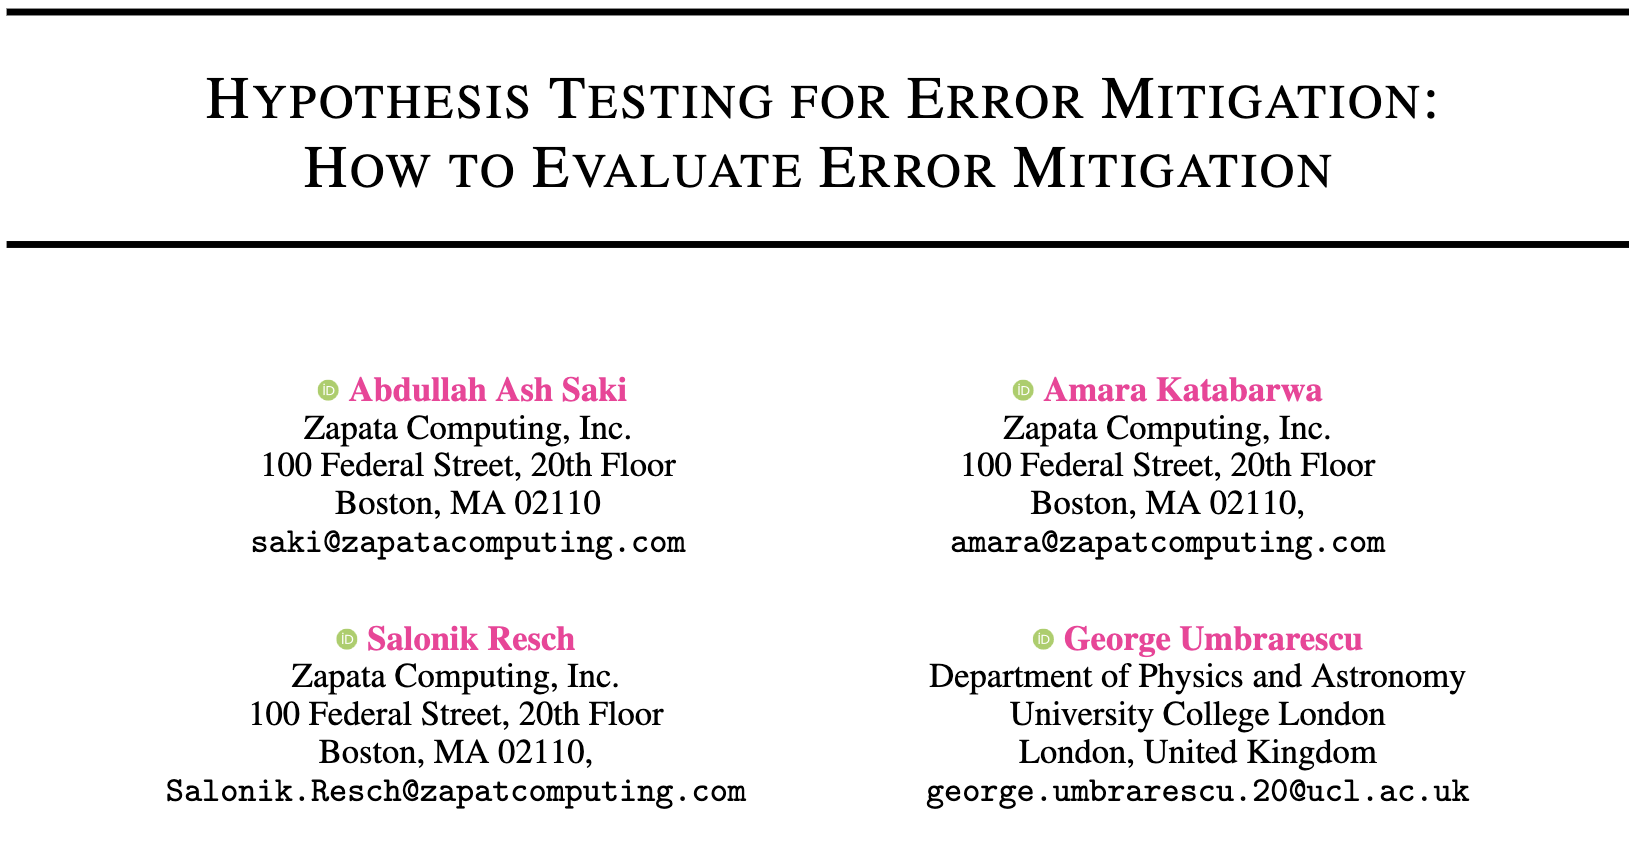
\includegraphics[width=0.8\textwidth]{paper.png}
	\end{figure}
	\begin{center}
		\url{https://arxiv.org/abs/2301.02690}
	\end{center}
\end{frame}

\begin{frame}{Overview}
	Two main questions:
	\begin{enumerate}[<+->]
		\item How can we understand ``stacking'' error mitigation techniques?
		\item How can we assess the tradeoffs associated with a variety of techniques in a way that captures overhead?
	\end{enumerate}
\end{frame}

\begin{frame}{Noise Estimation Circuits}
	\begin{quantikz}[column sep=0.38cm]
		& \gate{} & \ctrl{1} & \ctrl{2} & \qw      & \gate{} & \ctrl{1} & \ctrl{2} & \qw      & \gate{} & \qw \\
		& \gate{} & \targ{}  & \qw      & \ctrl{1} & \gate{} & \targ{}  & \qw      & \ctrl{1} & \gate{} & \qw \\
		& \gate{} & \qw      & \targ{}  & \targ{}  & \gate{} & \qw      & \targ{}  & \targ{}  & \gate{} & \qw
	\end{quantikz}$\longrightarrow$\begin{quantikz}[column sep=0.38cm]
		& \qw & \ctrl{1} & \ctrl{2} & \qw      & \qw & \ctrl{1} & \ctrl{2} & \qw      & \qw & \qw \\
		& \qw & \targ{}  & \qw      & \ctrl{1} & \qw & \targ{}  & \qw      & \ctrl{1} & \qw & \qw \\
		& \qw & \qw      & \targ{}  & \targ{}  & \qw & \qw      & \targ{}  & \targ{}  & \qw & \qw
	\end{quantikz}

	\begin{columns}<2>
		\begin{column}{0.3\textwidth}
			\begin{equation*}
				\expval{O} = \frac{\expval{O}_\text{noisy}}{\frac{\#b_{00\cdots 0}}{N}}
			\end{equation*}

		\end{column}
		\begin{column}{0.7\textwidth}
			\begin{center}
				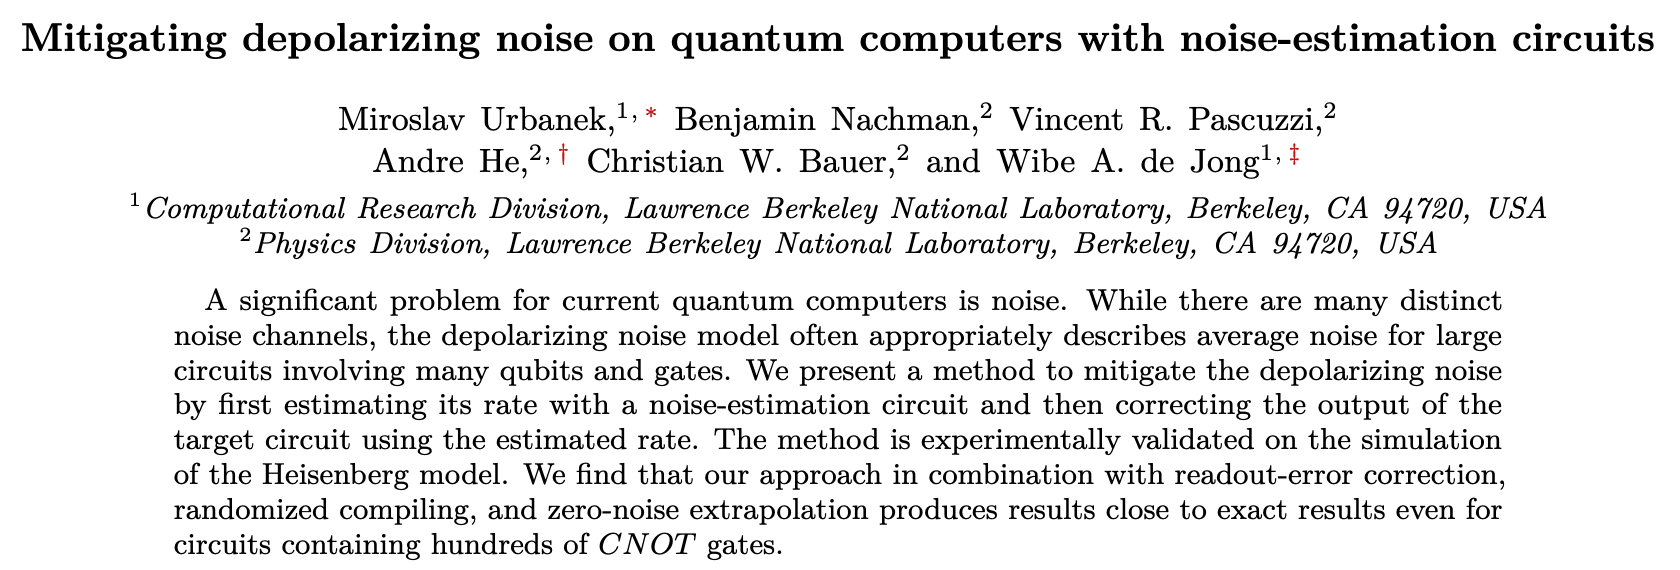
\includegraphics[width=0.9\textwidth]{noise-estimation.png}
				\url{https://arxiv.org/abs/2103.08591}
			\end{center}
		\end{column}
	\end{columns}
\end{frame}

\begin{frame}{Error Mitigation Pipelines}
	\begin{columns}
		\begin{column}{0.5\textwidth}
			\begin{center}
				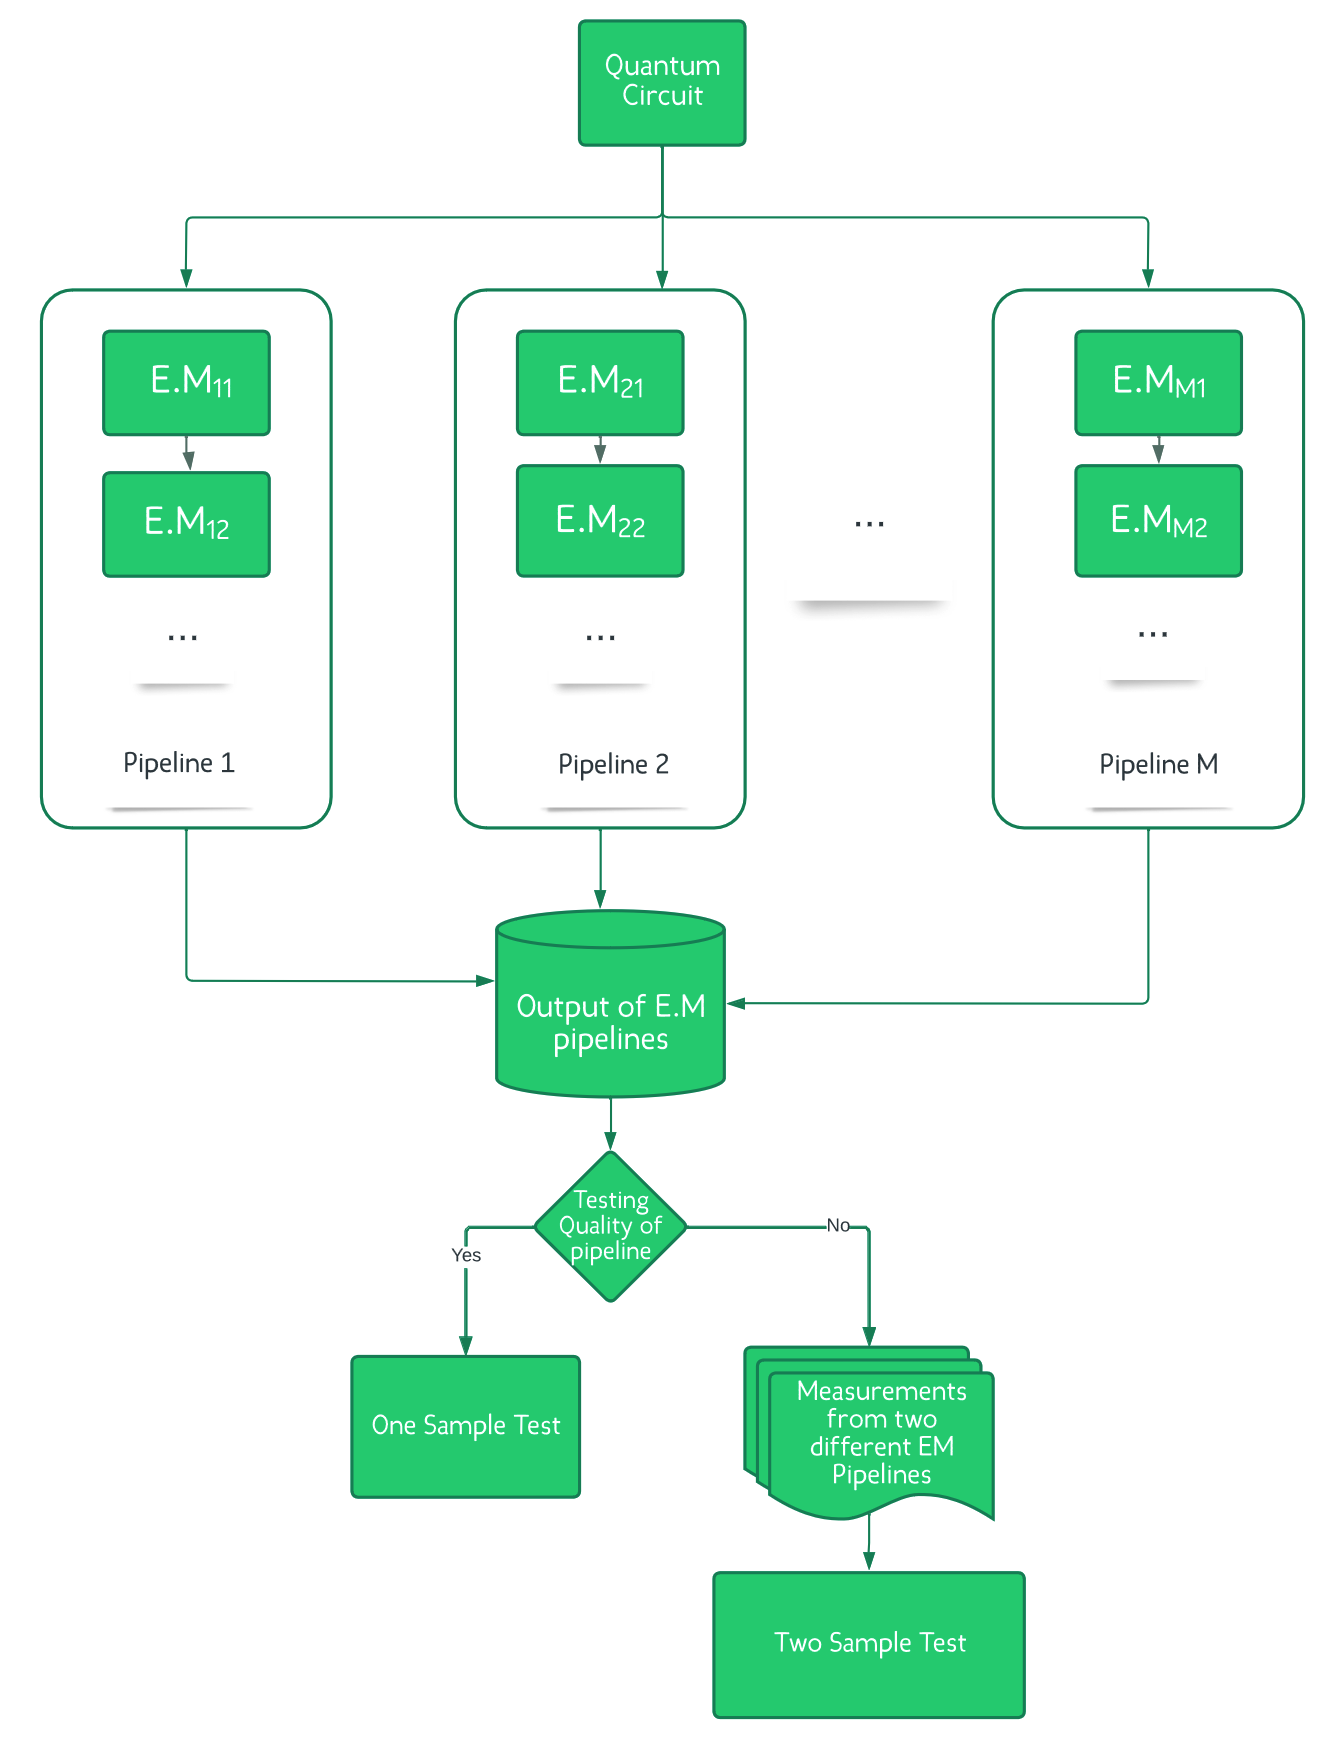
\includegraphics[height=0.9\textheight]{pipeline.png}
			\end{center}
		\end{column}
		\begin{column}{0.5\textwidth}
			\begin{table}[h]
				\centering\begin{tabular}{c l}
					Pipeline        & Composition                                             \\ \toprule
					$\mathcal{P}_1$ & \texttt{ZNE}                                            \\
					$\mathcal{P}_2$ & \texttt{ZNE} + \texttt{MEM}                             \\
					$\mathcal{P}_3$ & \texttt{ZNE} + \texttt{DD}                              \\
					$\mathcal{P}_4$ & \texttt{ZNE} + \texttt{DD} + \texttt{MEM}               \\
					$\mathcal{P}_5$ & \texttt{ZNE} + \texttt{RC}                              \\
					$\mathcal{P}_6$ & \texttt{ZNE} + \texttt{RC} + \texttt{MEM}               \\
					$\mathcal{P}_7$ & \texttt{ZNE} + \texttt{RC} + \texttt{DD}                \\
					$\mathcal{P}_8$ & \texttt{ZNE} + \texttt{RC} + \texttt{DD} + \texttt{MEM}
				\end{tabular}
			\end{table}

			$\mathcal{P}_i^{(E)}$ indicates extrapolation performed on scaled expectation values.
		\end{column}
	\end{columns}
\end{frame}

\begin{frame}[fragile]{Error Mitigation Methods}
	\begin{columns}
		\begin{column}{0.5\textwidth}
			\begin{enumerate}
				\item<1> Zero-Noise extrapolation
					\begin{itemize}
						\item Scale factors: \texttt{[1, 3, 5]}
						\item Folding methods: Global folding, \texttt{CNOT} folding
						\item Extrapolation methods: Linear, Quadratic
					\end{itemize}
				\item<2> Measurement Error Mitigation
					\begin{itemize}
						\item $C_\text{mitigated} = M^{-1}_\text{calib}\cdot C_\text{noisy}$
					\end{itemize}
				\item<3,4> Randomized Compiling
					\begin{itemize}
						\item Convert coherent errors into incoherent ones
					\end{itemize}
				\item<5> Dynamic Decoupling
					\begin{itemize}
						\item X-X sequence
					\end{itemize}
			\end{enumerate}
		\end{column}

		\begin{column}{0.5\textwidth}
			\only<1>{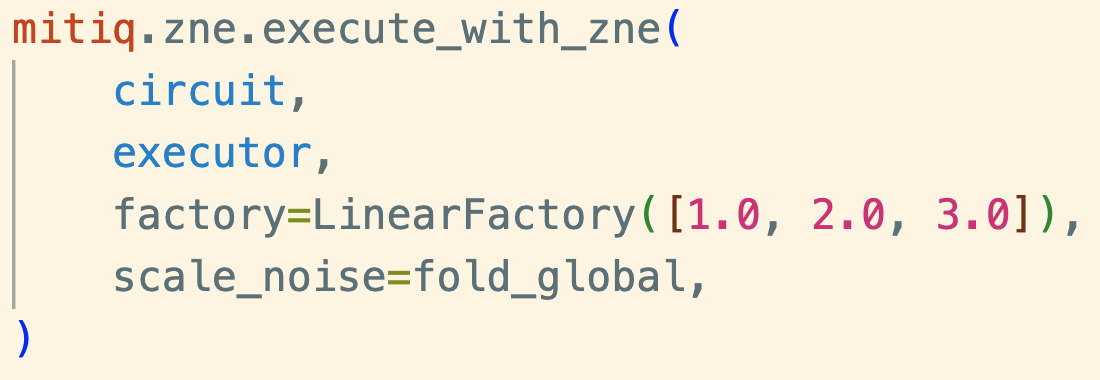
\includegraphics[width=\textwidth]{znecode.png}}

			\only<2>{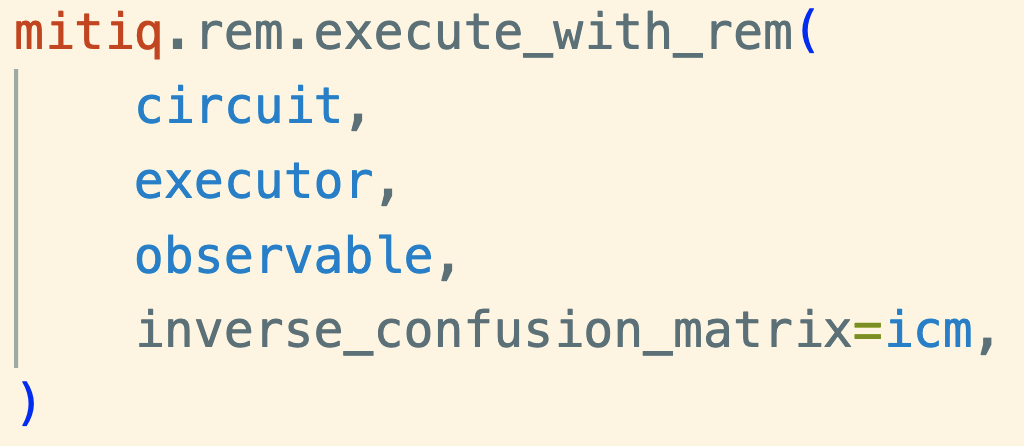
\includegraphics[width=0.9\textwidth]{remcode.png}}

			\only<3>{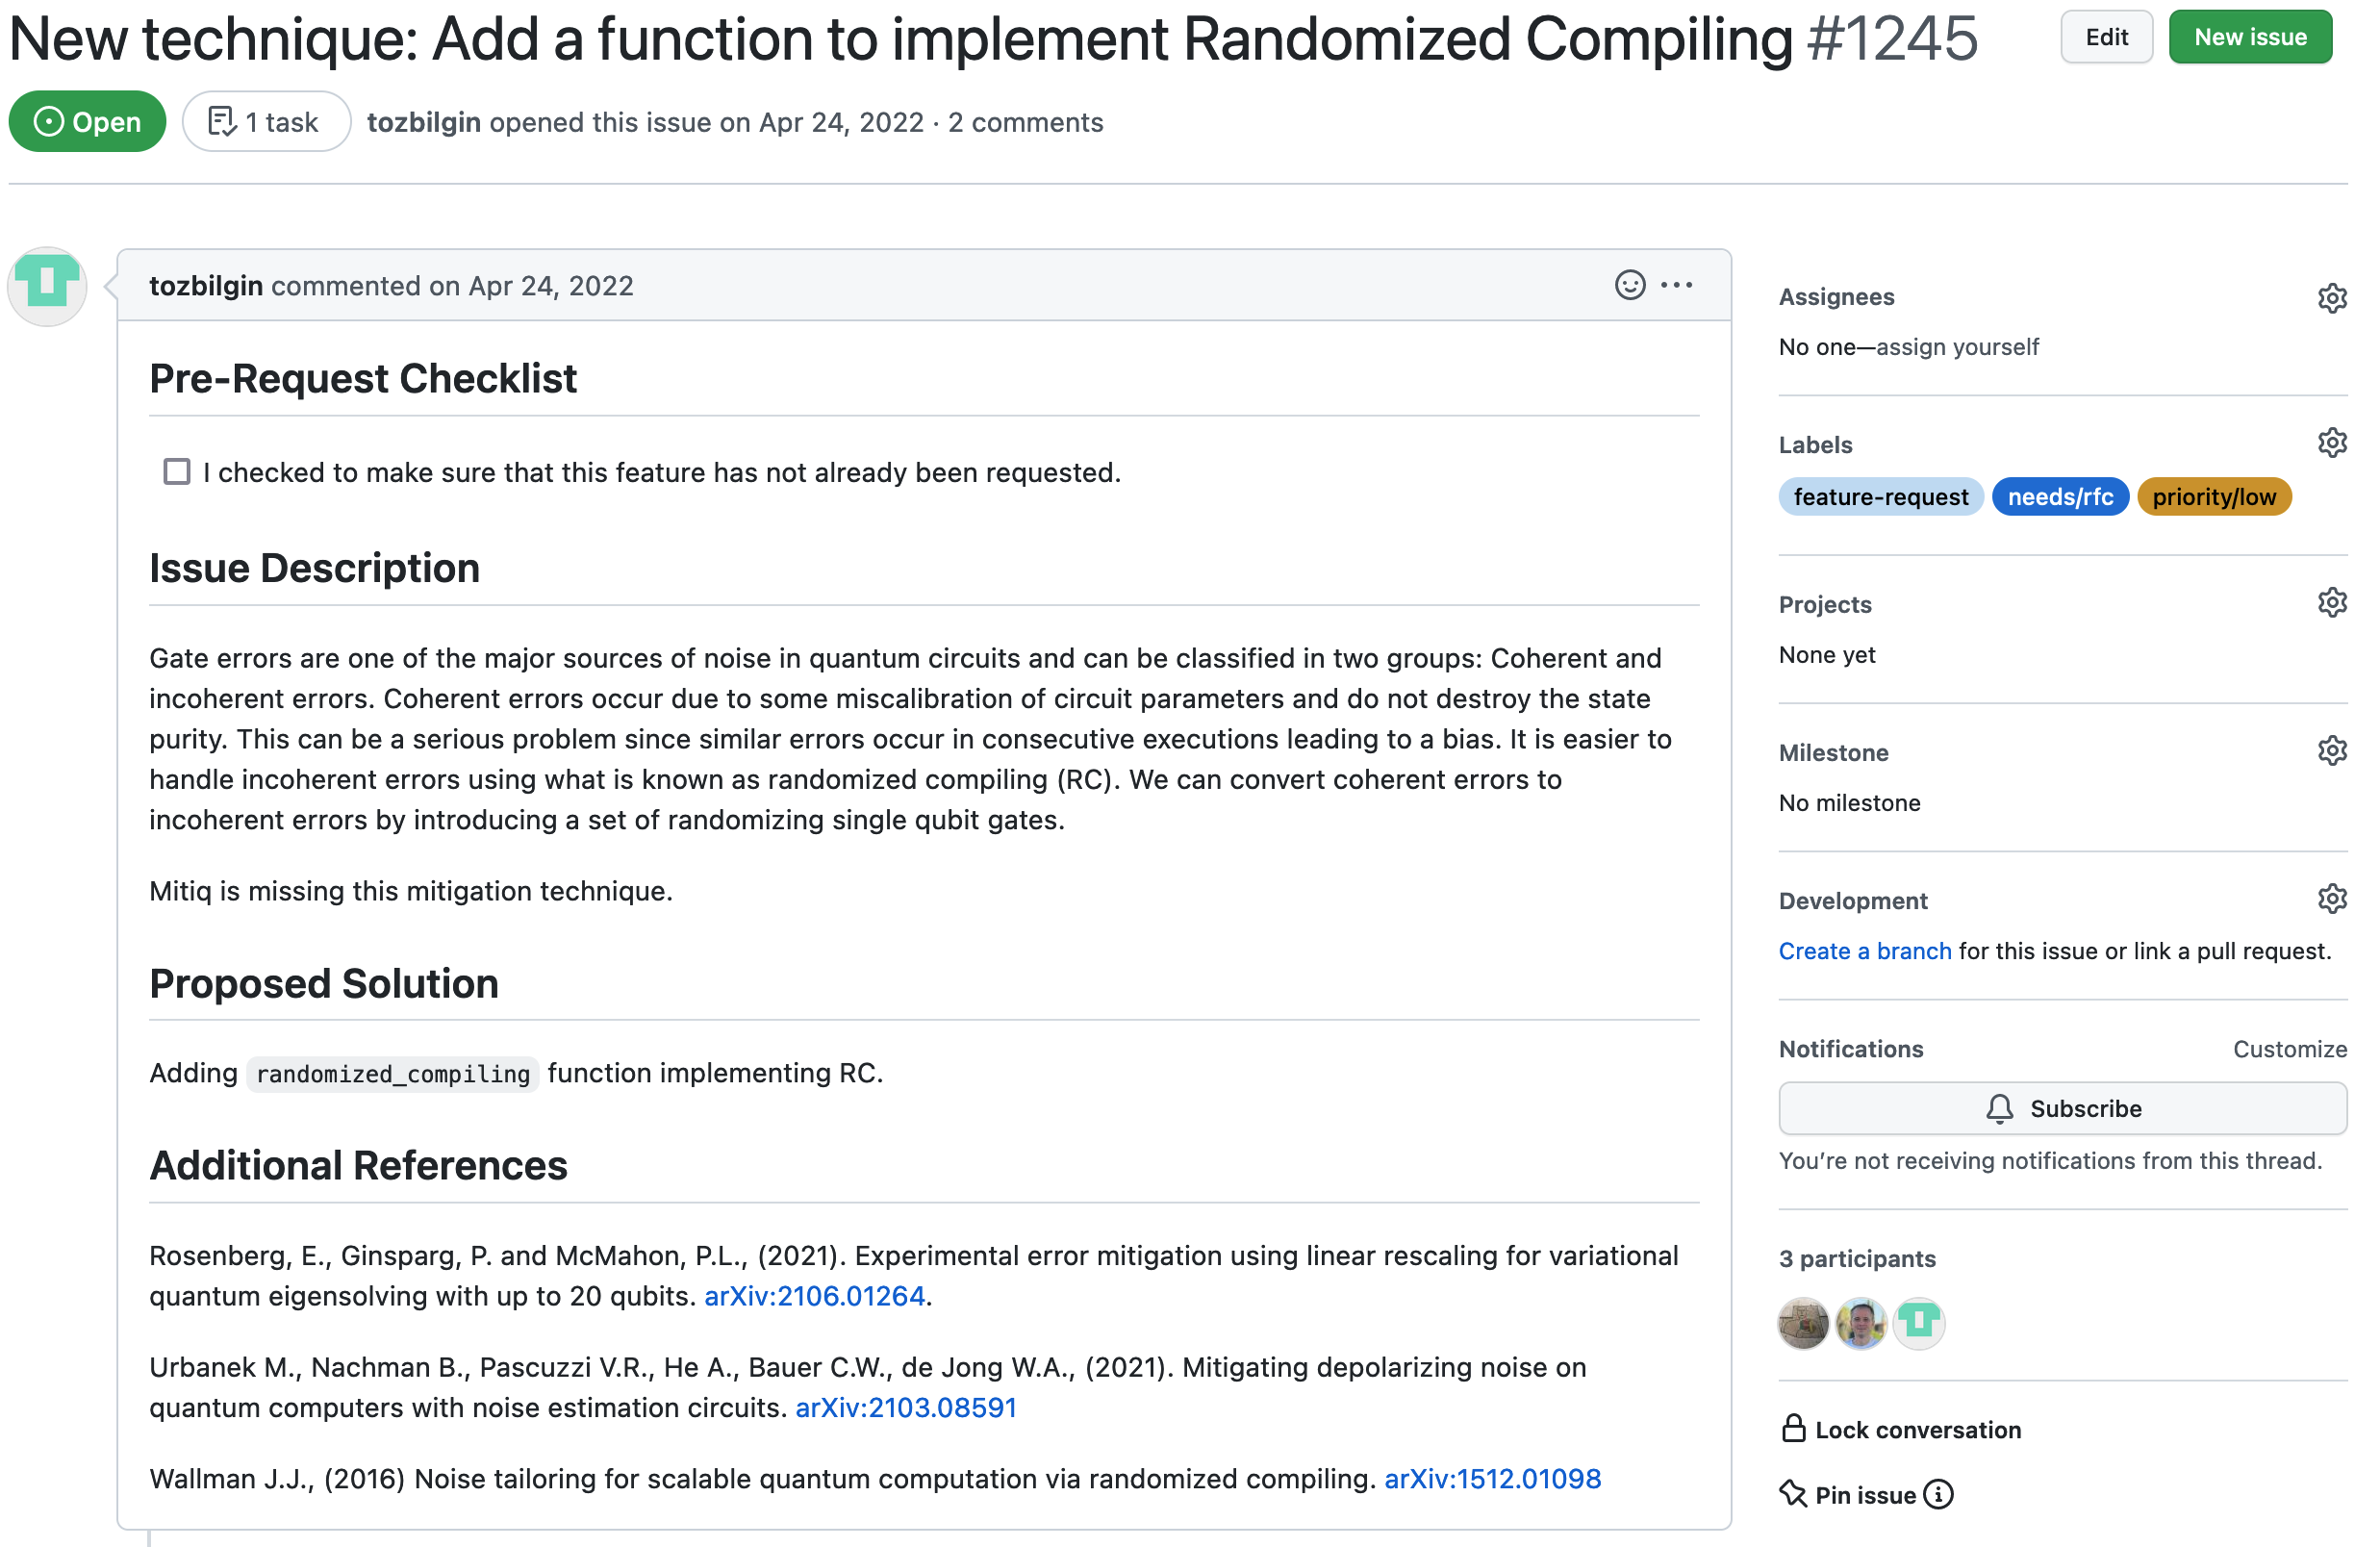
\includegraphics[width=\textwidth]{rc.png}}

			\only<4>{
				\begin{center}
					\begin{quantikz}[row sep=0.65cm]
						& \ctrl{1} & \qw \\
						& \targ{}  & \qw
					\end{quantikz}=\begin{quantikz}[row sep=0.3cm]
						& \gate{P} & \ctrl{1} & \gate{R} & \qw \\
						& \gate{Q} & \targ{}  & \gate{S} & \qw
					\end{quantikz}
					\vspace{0.5cm}
					\begin{tabular}{c c c c}
						$P$ & $Q$ & $R$ & $S$ \\ \toprule
						$I$ & $I$ & $I$ & $I$ \\
						$I$ & $X$ & $I$ & $X$ \\
						$I$ & $Y$ & $Z$ & $Y$ \\
						\vdots
					\end{tabular}
				\end{center}
			}

			\only<5>{
				\begin{center}
					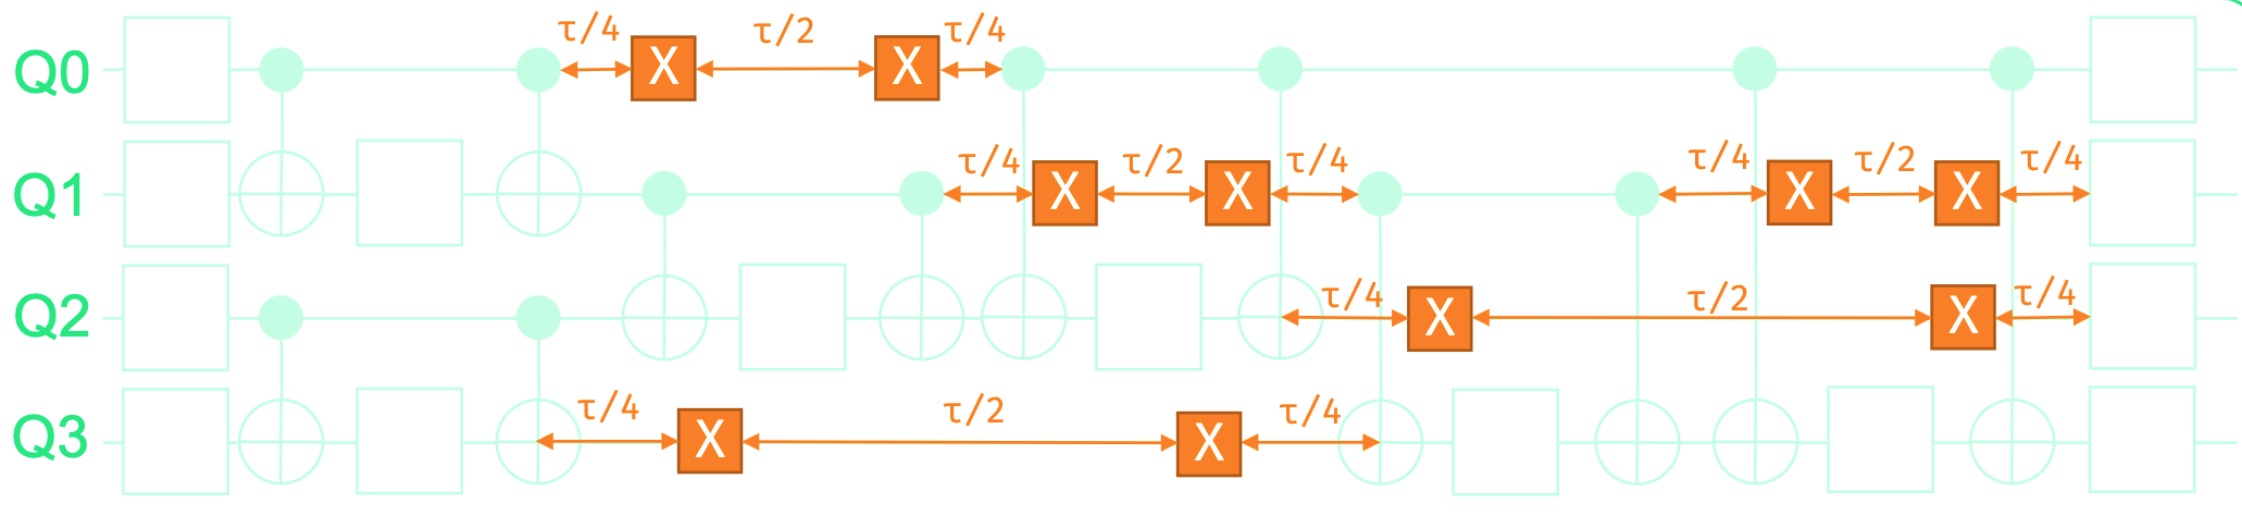
\includegraphics[width=\textwidth]{ddd.png}
					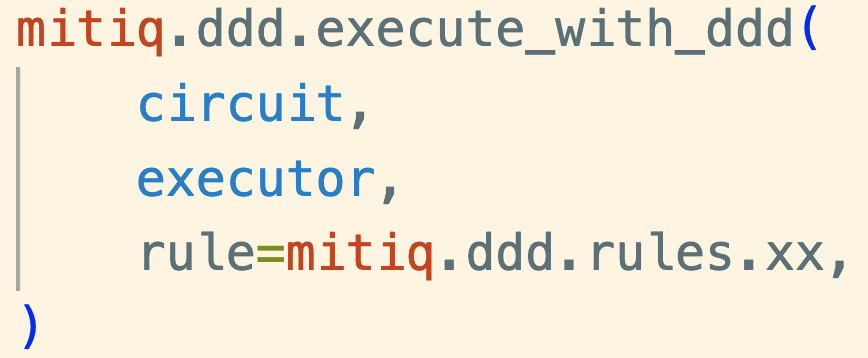
\includegraphics[width=0.8\textwidth]{dddcode.png}
				\end{center}
			}
		\end{column}
	\end{columns}
\end{frame}

\newcommand{\RZ}[1]{\scriptstyle{R_Z(#1)}}
\begin{frame}{Circuits}
	\begin{center}
		\begin{quantikz}[row sep=0.1cm, column sep=0.15cm]
			& \gate{H} & \ctrl{1} & \qw                & \ctrl{1} & \qw      & \qw                & \qw      & \ctrl{2} & \qw                & \ctrl{2} & \qw      & \qw                & \qw      & \ctrl{3} & \qw                & \ctrl{3} & \gate{\RZ{\beta}} & \qw \\
			& \gate{H} & \targ{}  & \gate{\RZ{\gamma}} & \targ{}  & \ctrl{1} & \qw                & \ctrl{1} & \qw      & \qw                & \qw      & \ctrl{2} & \qw                & \ctrl{2} & \qw      & \qw                & \qw      & \gate{\RZ{\beta}} & \qw \\
			& \gate{H} & \ctrl{1} & \qw                & \ctrl{1} & \targ{}  & \gate{\RZ{\gamma}} & \targ{}  & \targ{}  & \gate{\RZ{\gamma}} & \targ{}  & \qw      & \qw                & \qw      & \qw      & \qw                & \qw      & \gate{\RZ{\beta}} & \qw \\
			& \gate{H} & \targ{}  & \gate{\RZ{\gamma}} & \targ{}  & \qw      & \qw                & \qw      & \qw      & \qw                & \qw      & \targ{}  & \gate{\RZ{\gamma}} & \targ{}  & \targ{}  & \gate{\RZ{\gamma}} & \targ{}  & \gate{\RZ{\beta}} & \qw
		\end{quantikz}
	\end{center}

	Ten $(\gamma, \beta)$ pairs chosen to cover the possible ideal expectation values $(-0.62, 2)$.
\end{frame}

\begin{frame}{Figure of Merit}
	What's harder
	\begin{enumerate}
		\item running 1 circuit with 10,000 shots, or
		\item running 10 circuits with 1,000 shots each?
	\end{enumerate}

	% \begin{align*}
	% 	R                   & = T(1 + S)                                    \\
	% 	S                   & = -\sum_{i} p_{C_i} \ln(p_{C_i})              \\
	% 	T                   & = \sum_{i}N_{C_i}D_{C_i}Q_{C_i}^\text{norm}   \\
	% 	Q_{C_i}^\text{norm} & = \frac{Q_{C_i}}{Q_\text{max}}                \\
	% 	p_{C_i}             & = \frac{N_{C_i}D_{C_i}Q_{C_i}^\text{norm}}{T}
	% \end{align*}
	\begin{columns}
		\begin{column}{0.5\textwidth}
			\begin{align*}
				R       & = T(1 + S)                         \\
				S       & = -\sum_{i} p_{C_i} \ln(p_{C_i})   \\
				T       & = \sum_{i}N_{C_i}D_{C_i}           \\
				p_{C_i} & = \frac{N_{C_i}D_{C_i}}{T}         \\
				M       & = \frac{PSR(\%)}{\epsilon \cdot R}
			\end{align*}
		\end{column}
		\begin{column}{0.5\textwidth}
			\begin{align*}
				N_{C_i}  & = \text{number of shots for circuit } C_i \\
				D_{C_i}  & = \text{duration of circtui } C_i         \\
				\epsilon & = \text{median improvement factor (REM)}
			\end{align*}
		\end{column}
	\end{columns}

\end{frame}


\begin{frame}{Results}
	\begin{center}
		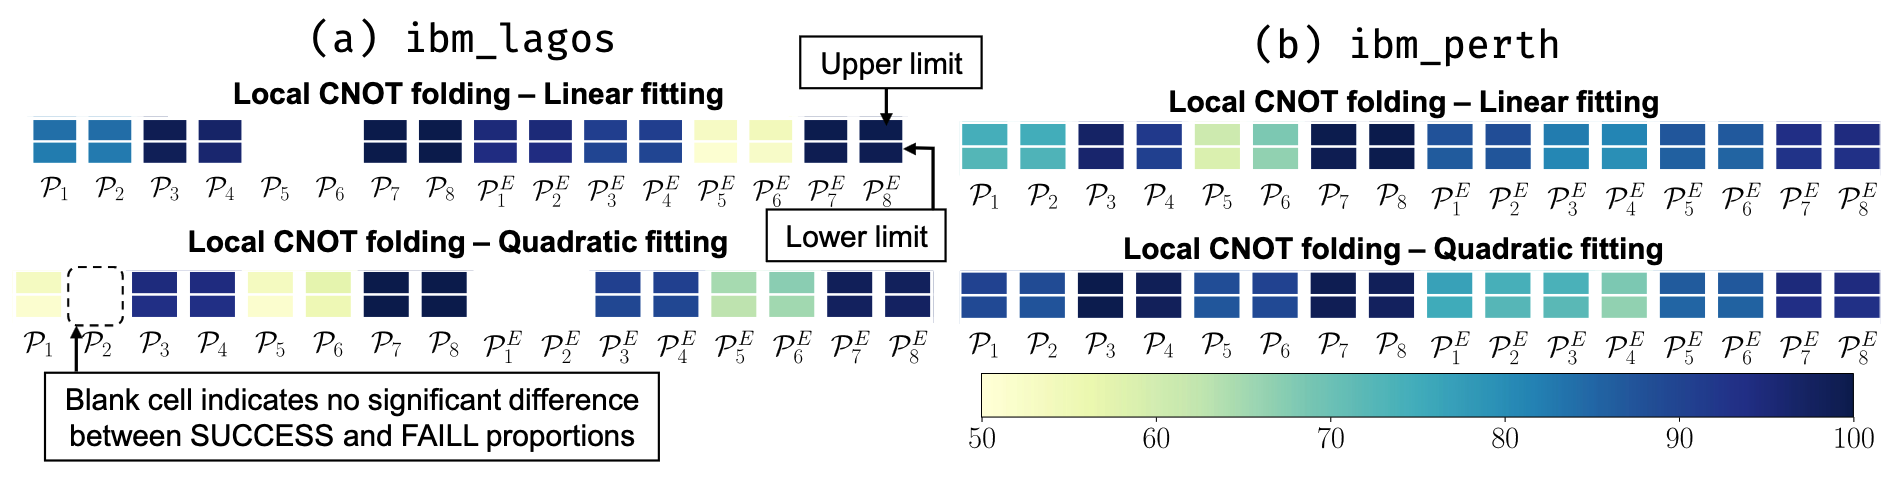
\includegraphics[width=0.8\textwidth]{results.png}
	\end{center}
	\begin{table}[h]
		\centering\begin{tabular}{c l}
			Pipeline        & Composition                                             \\ \toprule
			$\mathcal{P}_1$ & \texttt{ZNE}                                            \\
			$\mathcal{P}_2$ & \texttt{ZNE} + \texttt{MEM}                             \\
			$\mathcal{P}_3$ & \texttt{ZNE} + \texttt{DD}                              \\
			$\mathcal{P}_4$ & \texttt{ZNE} + \texttt{DD} + \texttt{MEM}               \\
			$\mathcal{P}_5$ & \texttt{ZNE} + \texttt{RC}                              \\
			$\mathcal{P}_6$ & \texttt{ZNE} + \texttt{RC} + \texttt{MEM}               \\
			$\mathcal{P}_7$ & \texttt{ZNE} + \texttt{RC} + \texttt{DD}                \\
			$\mathcal{P}_8$ & \texttt{ZNE} + \texttt{RC} + \texttt{DD} + \texttt{MEM}
		\end{tabular}
	\end{table}
\end{frame}

\begin{frame}{Results}
	\begin{center}
		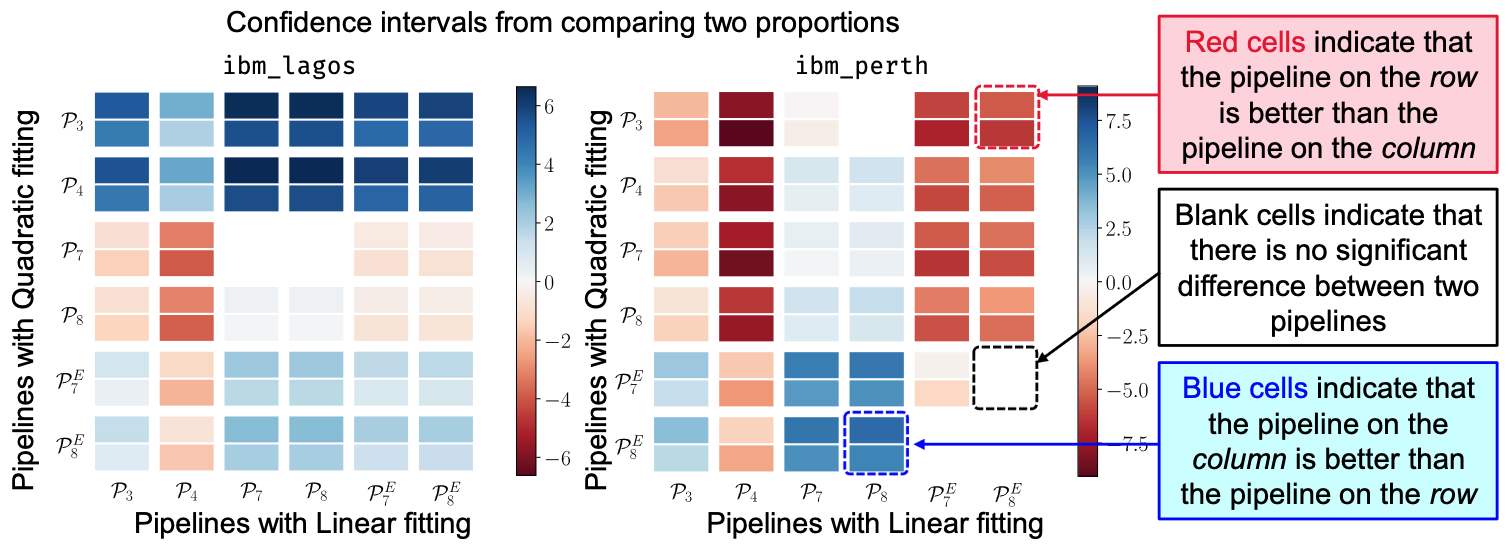
\includegraphics[width=0.9\textwidth]{comparisons.png}

		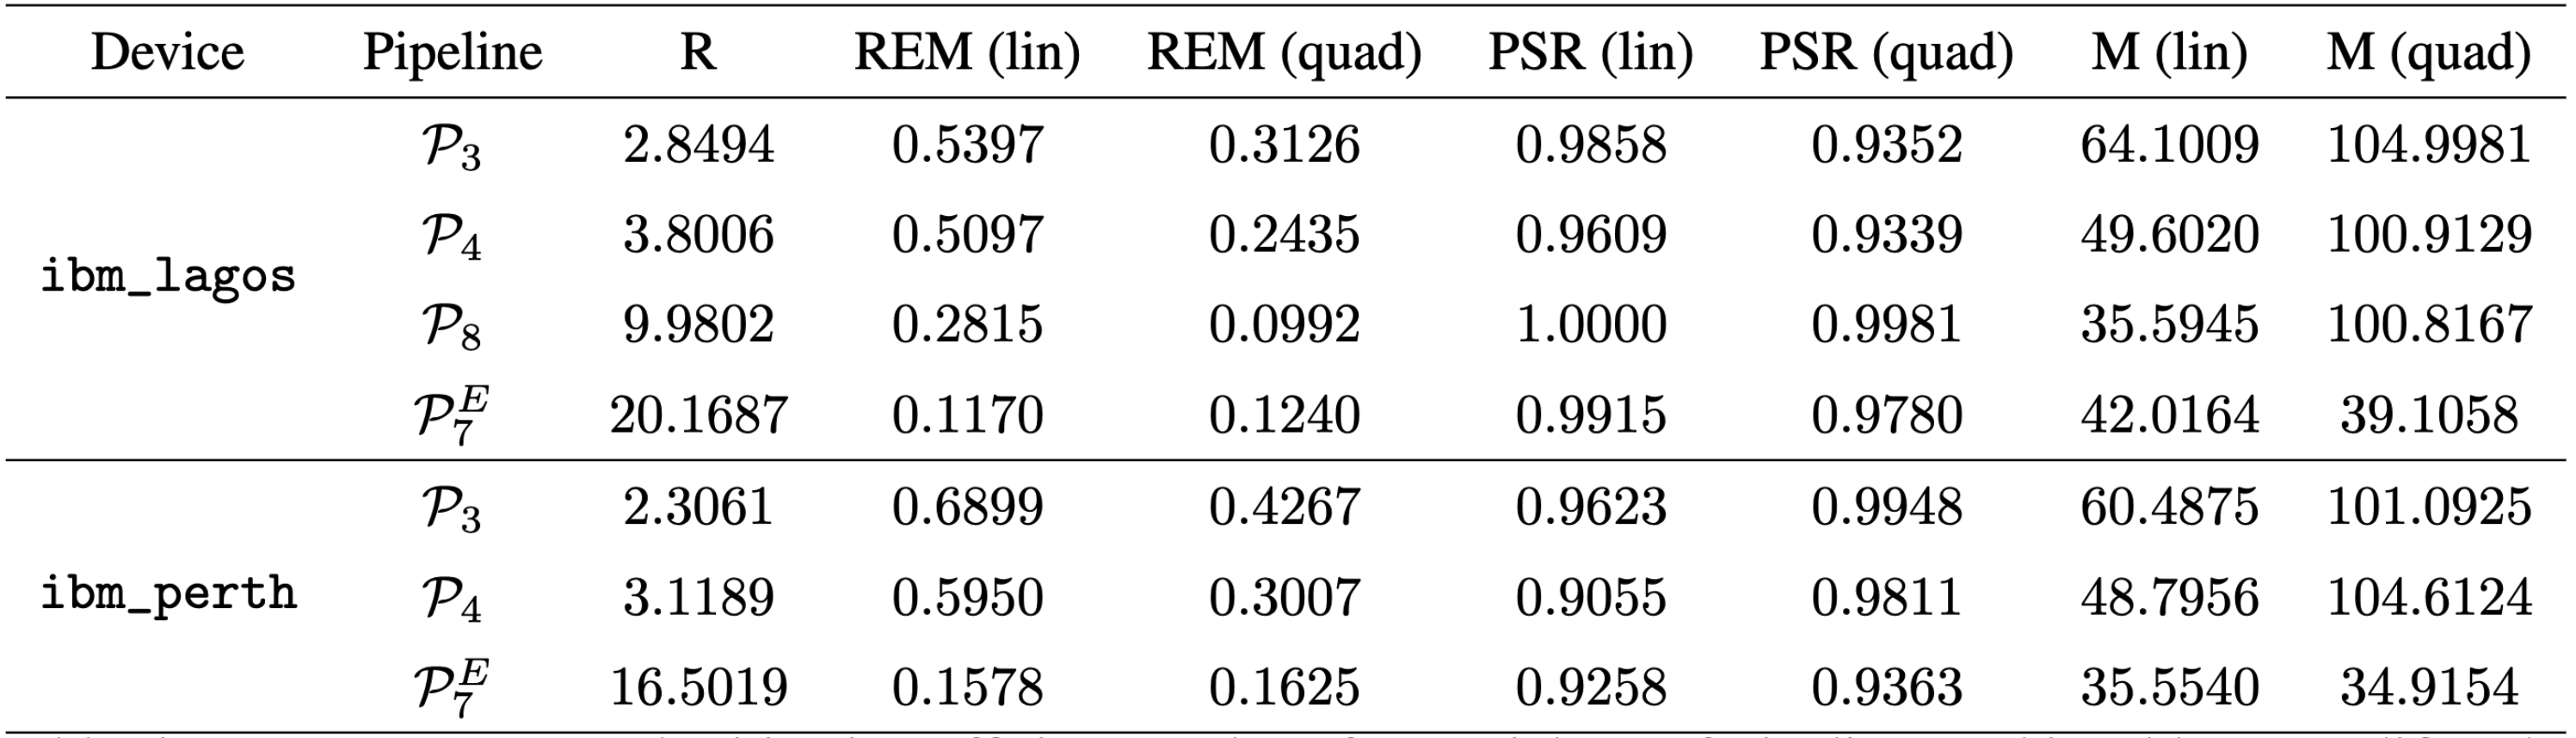
\includegraphics[width=0.8\textwidth]{table.png}
	\end{center}
\end{frame}

\begin{frame}{Results}
	\begin{center}
		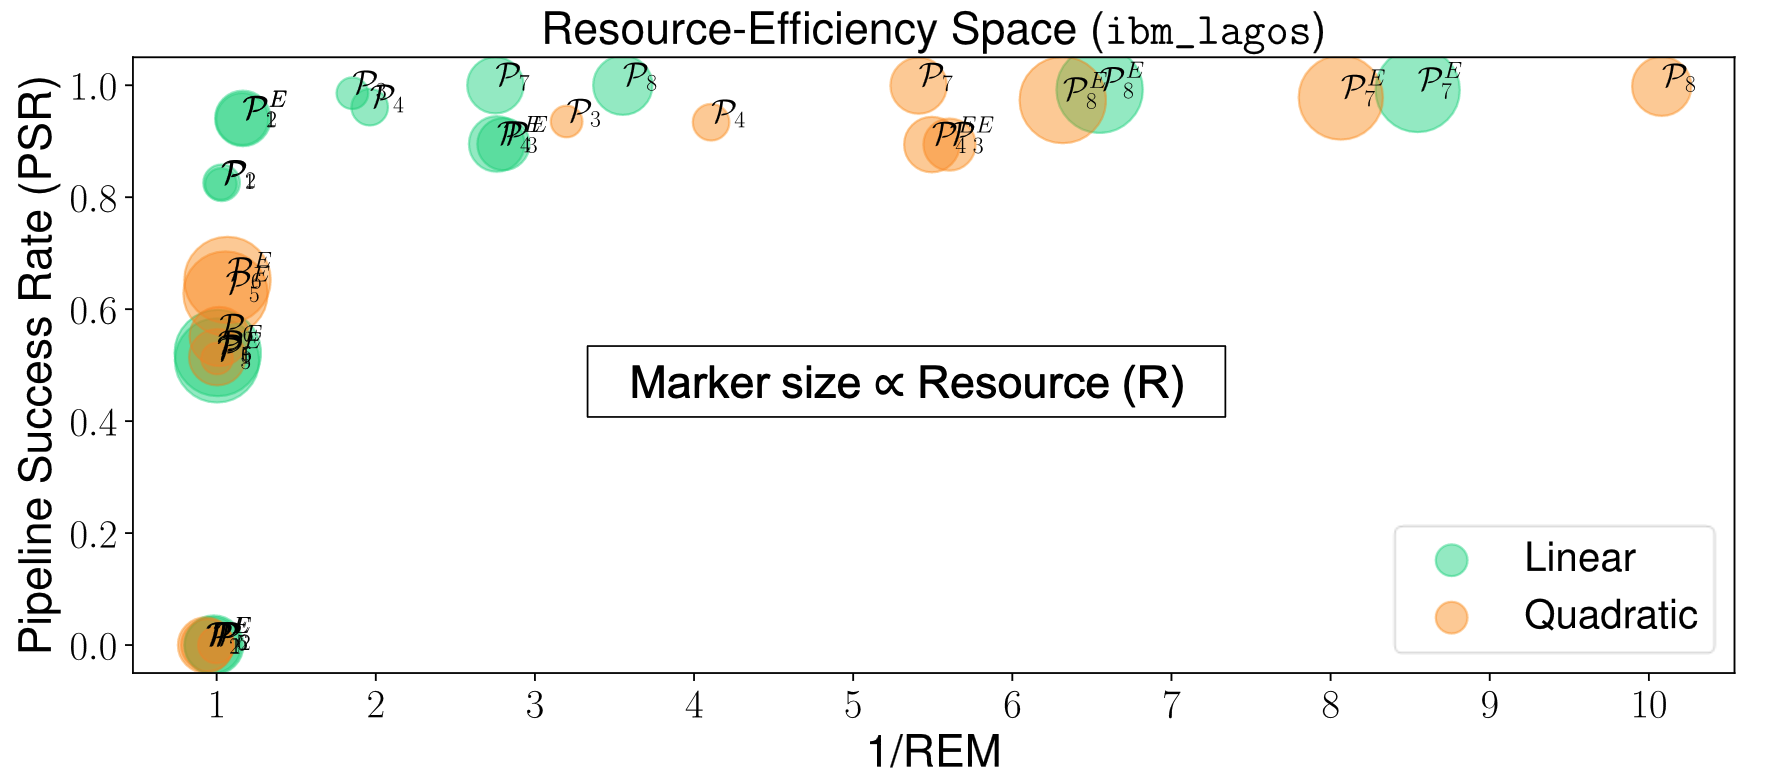
\includegraphics[width=0.65\textwidth]{psr1.png}

		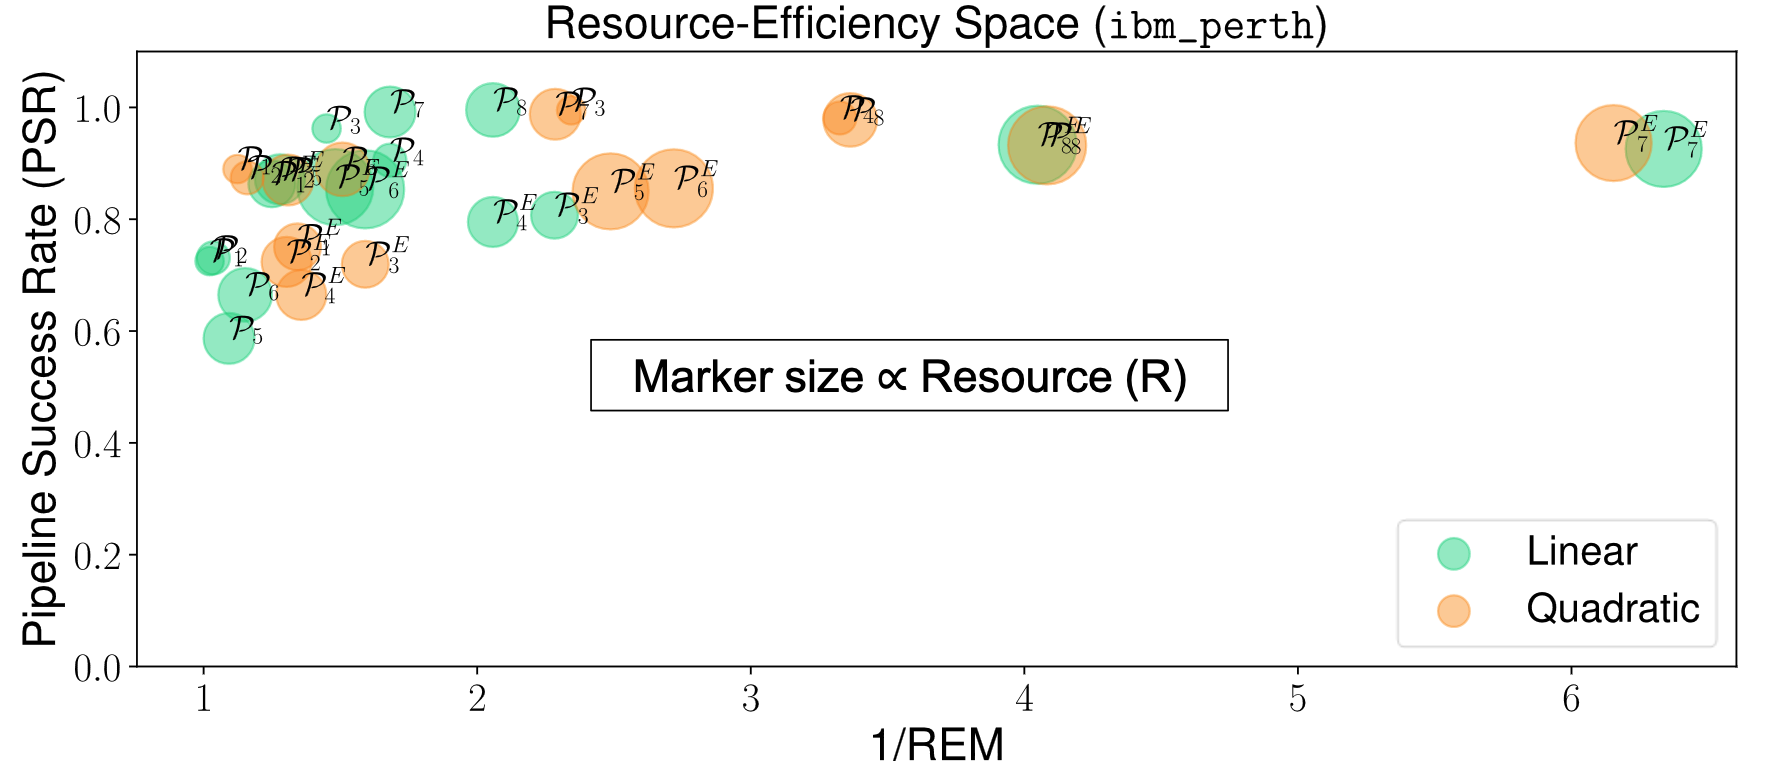
\includegraphics[width=0.65\textwidth]{psr2.png}
	\end{center}
\end{frame}


\begin{frame}[standout]
	Thank you!
\end{frame}

\end{document}
